%\documentclass{article}
\documentclass[12pt]{article}
\usepackage{times}
%\usepackage{natbib}
%\usepackage{multicol}
\RequirePackage{natbib}
\usepackage{amsmath, amssymb, fullpage, amsthm, array, algorithm2e,graphicx,asa}
%\usepackage[dvips]{graphics}

%\usepackage{hyperref} % for hyper reference

\graphicspath{{images/}}
\usepackage{color}
\newcommand{\blue}[1]{{\color{blue} #1}} %MM
\newcommand{\red}[1]{{\color{red} #1}} 
\newcommand{\green}[1]{{\color{green} #1}} %DC

\definecolor{orange}{rgb}{1,0.5,0}
\newcommand{\hh}[1]{{\color{orange} #1}} %HH

% \usepackage{pifont} % this package is used to print check mark \checkmark
% \linespread{1.6} % factor 1.6 = double space

\usepackage{setspace}
\doublespacing



\setlength{\oddsidemargin}{0in}
\setlength{\evensidemargin}{0in}
\setlength{\textwidth}{6.5in}
\setlength{\topmargin}{-0.4in}
\setlength{\textheight}{9in}
\evensidemargin 
\oddsidemargin

\newtheorem{thm}{Theorem}[section]
\newtheorem{dfn}{Definition}[section]
\newtheorem{cor}{Corollary}[thm]
\newtheorem{con}{Conjecture}[thm]
\newtheorem{lemma}[thm]{Lemma}

%\topmargin -0.10in   % when making pdf
%\textheight 9.15in  % when making pdf

\pdfminorversion=4 % as instructed by JASA file upload


\begin{document}


\begin{table}[hbtp]
%\renewcommand\thetable{}
\caption{Selection of 10 lineups for a person to evaluate in the simulation experiment with discrete covariate described in section 5.1 of the paper.} 
\centering
\begin{tabular}{c c c c  c c c}
\hline\hline
Difficulty& \multicolumn{3}{c}{parameter combination}& Number of evaluations &Total number  & number of lineups\\
 \cline{2-4}
level & $n$ & $\sigma$ & $\beta$ &required($n_{\gamma}$) & of lineups & randomly shown \\
\hline
easy&100& 5&8 & 1& 12 & 1\\
&100&12&16 &1&&\\
&300& 5&5 &1&&\\
&300&12&10 &1 &&\\
\hline
medium&100& 5&3 &203 & 9 &2\\
&300& 5&2, 3 & 97, 1&&\\
\hline
hard&100&12&3, 8, 10 & 277, 126, 23& 18 &6\\
&300& 5&1 & 371 &&\\
&300&12&3, 5& 375, 74 &&\\
\hline
mixed&100& 5&1, 5, 0& 214, 2, 73 & 21 &1\\
&100&12&1& 100& &\\
&300& 5&0 & 73&&\\
&300&12&7, 1& 2, 152&&\\
\hline
Total &&&&&60&10\\
\hline
\end{tabular}
\label{tbl:dist_lineup1}
\end{table} 

\section{Proof of the Lemma}

\begin{proof}
%We will now make use of properties of the data going into the lineup and assume that the properties are reflected in the lineup display:

 By definition  

$$p_D=Pr\left(|t| \ge t_{obs} \mid H_0\right)=1-F_{|t|}(t_{obs}) \ \ \Rightarrow \ \  |t_{obs}|=F_{|t|}^{-1}(1-p_D)$$

%Now suppose $F_{|t|}(.;\delta)$ denotes the distribution function of an absolute value of $t$, the conventional test statistic.
%, with non-centrality parameter $\delta$. 
\noindent Then the distribution function of the $p$-value, $p_D$, under $H_0$, is uniform, since:  
\begin{eqnarray}\label{dist_p}
F_{p_D}(p) &=& Pr(p_D \le p)=1-Pr(1-p_D \le 1-p) \nonumber \\
  &=& 1-Pr\left(F_{|t|}^{-1}(1-p_D) \le F_{|t|}^{-1}(1-p) \right) \nonumber \\
  &=& 1-Pr\left(|t_{obs}| \le F_{|t|}^{-1}(1-p)\right) \nonumber \\
  &=&%\left\{ \begin{array}{ll}
          1-F_{|t|}\left( F_{|t|}^{-1}(1-p)\right)=p \mbox{ ; under $H_0$} 
 %         1-F_{|t|}( F_{|t|}^{-1}(1-p); \delta) &\mbox{ ; under $H_1$} 
%       \end{array} \right.     
\end{eqnarray}

%Thus the density of $p_D$ is Uniform(0,1)  under $H_0$. As noted by \cite{Ruppert:2007}, under $H_1$ the density of $p_D$ $$f_{p_D}(p_D; \delta)= \frac{f_{|t|}(F_{|t|}^{-1}(1-p_D);\delta)}{f_{|t|}(F_{|t|}^{-1}(1-p_D))}$$ derived from equation \eqref{dist_p}  is a right skewed distribution.  



Let $p_{0,i}$, $i=1, ..., m-1$ denote the  $p$-values associated with data corresponding to the $m-1$ null plots. Since this data is generated consistently with the null hypothesis,  the $p$-values are independent and  follow a standard Uniform distribution, $p_{i,0} \sim U[0,1], i= 1, ..., m-1$. The minimum $p_0 = \min_{1 \le i \le m-1}  \ p_{0,i}$ then follows a Beta distribution with shape parameters 1 and $m-1$, and corresponding distribution function 
\[
F_{p_0} (x) =  1- (1- x) ^{m-1}  \text{ for } x \in [0,1].
\]

\noindent Thus
\begin{eqnarray*}
P(p_D < p_{0}) &=& 1 - P(p_{0} \le p_D) = 1- \int_0^1  P(p_{0} \le p_D \mid p_D=t) f_{p_D}(t) dt   \\
&=& 1 - \int_0^1 F_{p_{0}}(t) f_{p_D}(t) dt = 1 - \int_0^1 f_{p_D}(t) dt + \int_0^1 (1-t)^{m-1} f_{p_D}(t) dt  \\
&=&  E\left[ (1 - p_D)^{m-1}\right].
\end{eqnarray*}


%\noindent This proves the statement above. 
%We further see:
%\[
%E\left[ (1 - p_D)^{m-1}\right] =  \sum_{k=0}^{m-1} {m-1 \choose k} (-1)^k E[p_D^k] = 1-(m-1)E[p_D] + O(E[p_D^2]).
%\]


% If the density of $p$-value is very right skewed, the expectation term would be large. The distribution function would be highly right skewed when there would be strong signal in the data plot.Thats where the distribution function of $p$-value under alternative comes in. Should we add that in Equation \ref{dist_p}? )},
%conversely, as $m$, the number of choices given in the lineup, goes up the probability to pick the data plot  goes down. 
%}
%\blue{This shows that the lineup size $m$ has an effect on the power of the visual test: it is the $m-1$th moment of the distribution of $1-p_D$. 

%
%
%
%Let us think of a lineup as a head-to-head comparison of the test statistic and $m-1$ null plots. 
%%Let the data plot have a $p$-value of $p_D$, and the null plots $p$ values of $p_{0, i}$ with $1 \le i \le m-1$.
%We know that for each comparison the probability that the data, on which the plot is based, has the smaller $p$ value is 
%\begin{eqnarray*}
%P(p_D < p_{0,i}) &=& 1 - P(p_{i,0} \le p_D) = 1- \int_0^1  P(p_{i,0} \le p_D \mid p_D=t) f_{p_D}(t) dt =  \\
%&=& 1 - \int_0^1 F_{p_{0,i}}(t) f_{p_D}(t) dt = 1 - \int_0^1 t f_{p_D}(t) dt = 1 - E[p_D],
%\end{eqnarray*}
%which, in particular, is independent of $p_{0,i}$ for all $i$.
%
%Let us make the assumption that an observer is able to identify  the chart corresponding to the data with the smallest $p$-value. Further we will assume that all observers  have the same ability in identifying the data plot.
%
%With that, we define $Z$  as the number of null plots in a lineup, for which the $p$-value $p_{0,i}$ is smaller than $p_D$.  
%
%Then $Z \sim B_{m-1, E[p_D]}$, and the probability that an observer will pick the data plot in a given lineup is 
%\[
%P(Z=0) = \left(1 - E[p_D] \right)^{m-1} = P(p_D \le p_0), \ \ \ \text{ where } p_0 = \min_{1 \le i \le m-1}  \ p_{0,i}.
%\]
\end{proof}



\section{Data Cleaning}

Following six approaches have been examined to clean the data.  Table \ref{tbl:summary} displays number of subjects and there total evaluations in each screening criteria. For our paper we picked criteria six.

\begin{enumerate}
\item {\bf Include all participants} and their evaluations.
\item Exclude all participants' evaluations, who did {\bf not} share their {\bf demographic information} (age, gender education level -- all three pieces of information are either missing or all present).
\item Exclude participants' records, if {\bf none of the evaluations}  correctly identified the data plot -- every participant was shown a range of `easy' lineups.
\item Include participants' records, if   {\bf at least 20 percent} of the evaluations are {\bf correct}  -- based on ten evaluations per participants, two correct evaluations are significant evidence against a person just guessing.
\item Include participants' records, if at least {\bf 50\% of all very easy (p-value $<$ 0.0002) lineups are correct} .
\item Use easy lineups as {\bf reference charts}: sample one easy lineup from a person's records. If that lineup is evaluated {\bf correctly}, include all (other) lineups of that person, otherwise exclude all lineup evaluations by this participant.
\end{enumerate}


The power curves obtained by fitting mixed model to the data for all the experiments applying different screening criteria are shown in Figure \ref{fig:power_screening_subject}. This shows how the screening criteria may affect the results. The corresponding power curves of conventional test are also shown. Notice that no mater what criteria we apply the result does not change much for experiment 2.  % Also, estimated power curve with criteria 5 for experiment 3 is above the conventional test power curve.


%\begin{figure}[hbtp]
%   \centering
%       \scalebox{0.70}{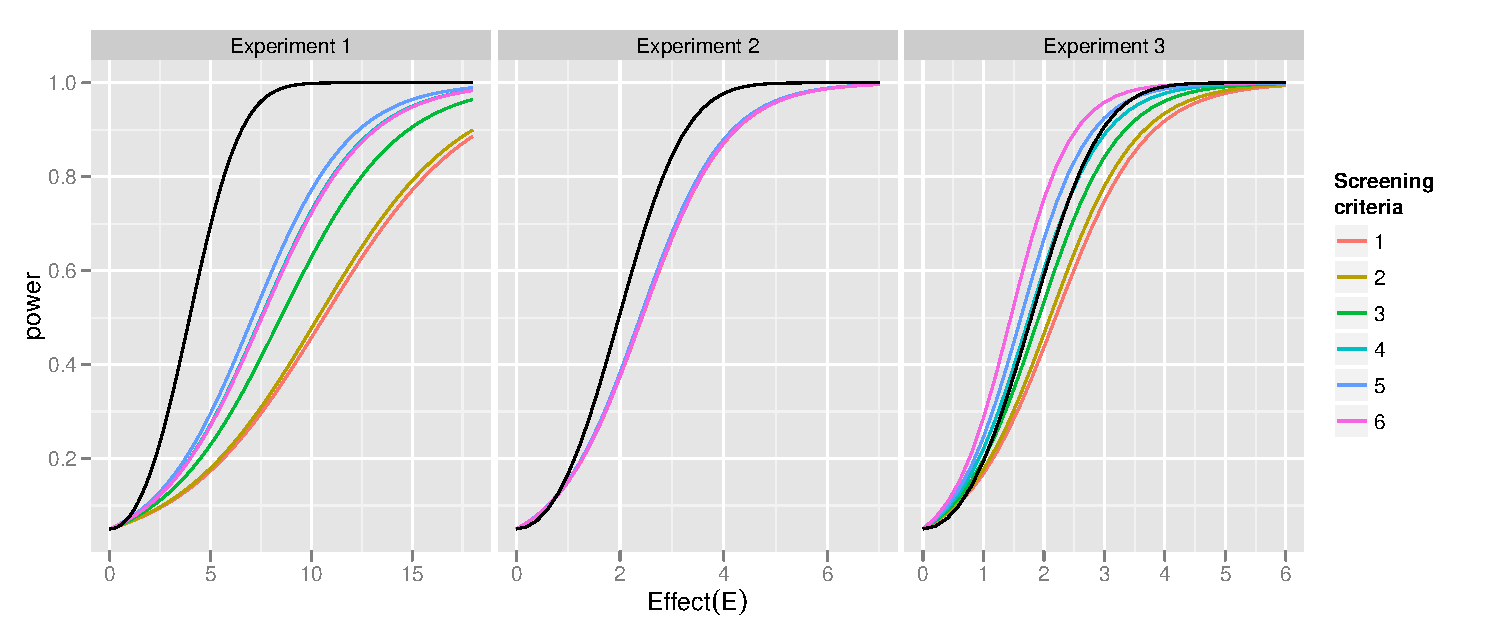
\includegraphics{power_screening.pdf}}
%       \caption{The overall power estimated from mixed model  for each screening criteria are shown. The corresponding power curve for conventional test is shown for comparison.}
%       \label{fig:power_screening}
%\end{figure}

\begin{figure}[hbtp]
   \centering
       \scalebox{0.70}{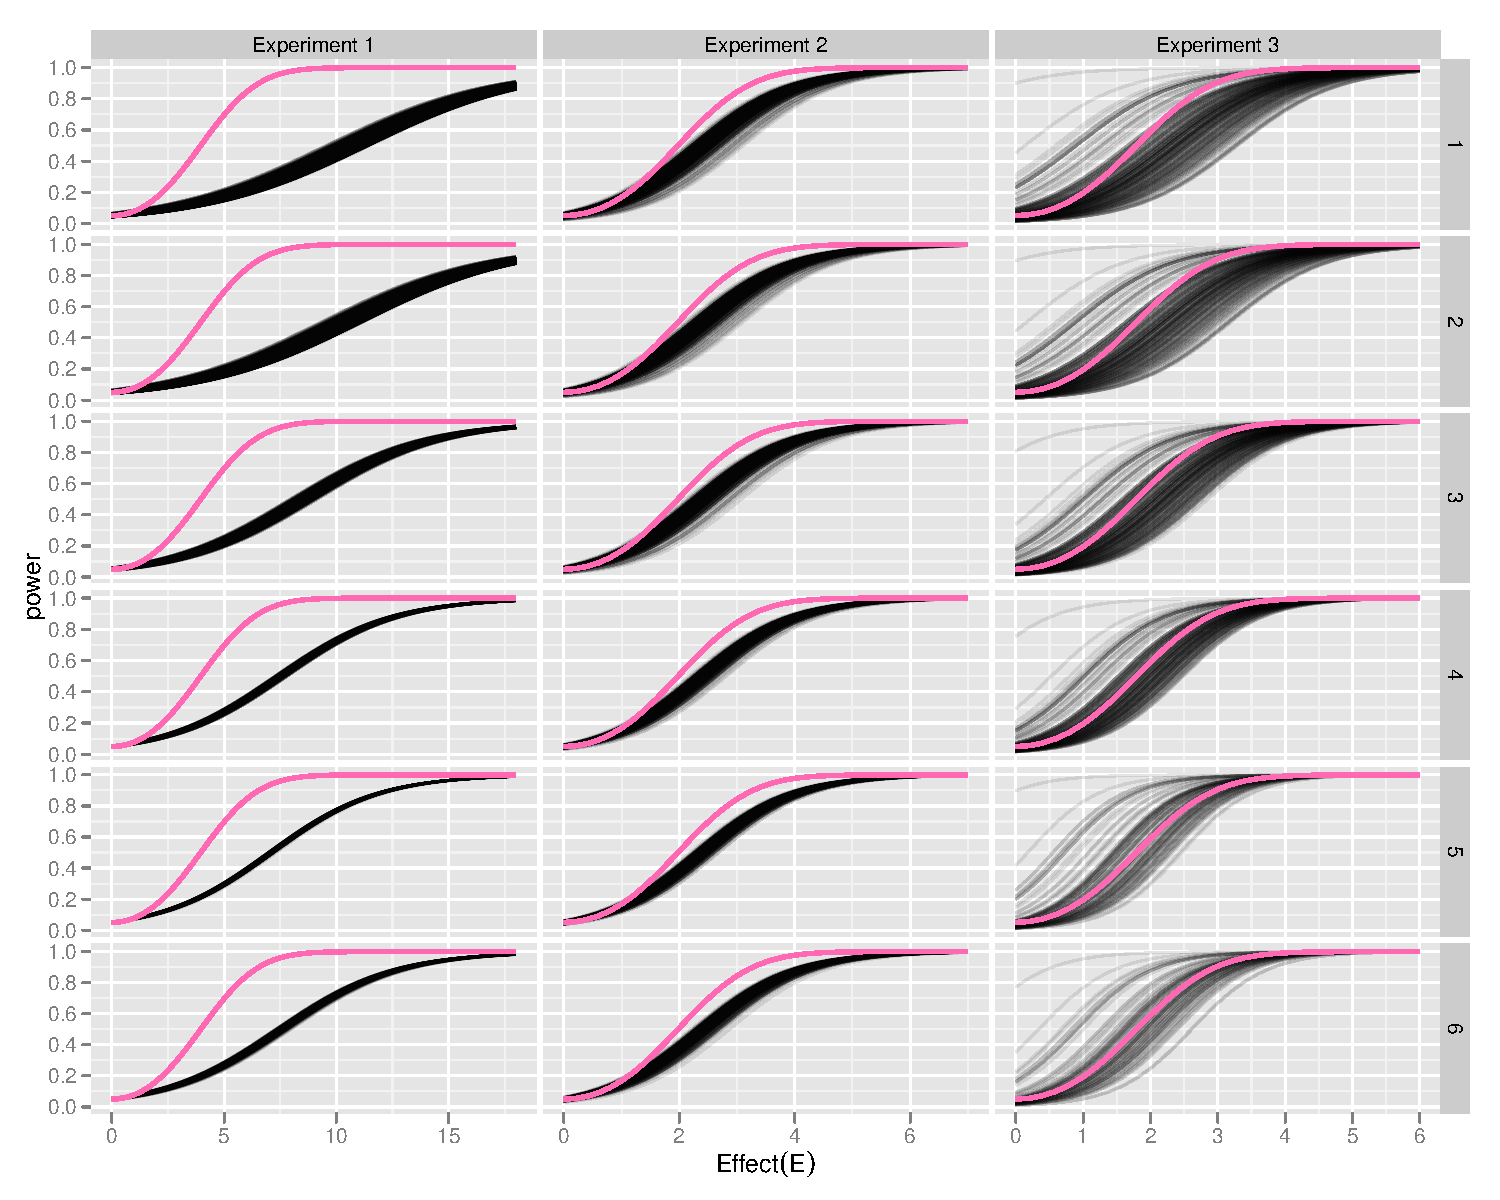
\includegraphics{power_screening_subject.pdf}}
       \caption{The subject specific power estimated from mixed model for all the six screening criteria are shown. The corresponding power curves for conventional test is shown for comparison.}
       \label{fig:power_screening_subject}
\end{figure}


\begin{table}[hbtp]
\caption{Number of unique subjects and their total feedbacks after applying six screening process on all three experimental data sets. 
Note that in some of the lines the number of male and female participants does not add up to the total number of participants. This is due to missing demographic information. }
\begin{center}
\begin{tabular}{rrrrr|rrrr|rrrr}
  \hline
Screening &  \multicolumn{4}{c} {Experiment 1}  & \multicolumn{4}{c} {Experiment 2}  & \multicolumn{4}{c} {Experiment 3} \\
 \cline{2-5}  \cline{6-9}   \cline{10-13}
criteria & Subj & Male & Fem & Total & Subj & Male & Fem & Total & Subj & Male & Fem & Total \\ 
  \hline
1 & 520 & 264 & 201 & 4914 & 390 & 203 & 182 & 4603 & 257 & 166 &  84 & 2830 \\ 
  2 & 465 & 264 & 201 & 4624 & 385 & 203 & 182 & 4558 & 250 & 166 &  84 & 2782 \\ 
  3 & 384 & 200 & 165 & 4187 & 384 & 199 & 181 & 4573 & 227 & 147 &  78 & 2648 \\ 
  4 & 318 & 168 & 135 & 3395 & 378 & 195 & 179 & 4492 & 205 & 133 &  72 & 2393 \\ 
  5 & 277 & 139 & 124 & 3008 & 374 & 193 & 177 & 4451 & 185 & 122 &  63 & 2121 \\ 
  6 & 239 & 121 & 107 & 2317 & 351 & 185 & 164 & 3858 & 156 & 106 &  50 & 1681 \\ 
   \hline
\end{tabular}
\end{center}
\label{tbl:summary}
\end{table}


\end{document}
